\renewcommand{\thechapter}{4}

\chapter{The Combined Energy Scale}
\label{Ch:E_Scale_Cal}

The ratio of the charge (S2) to light (S1) signals provide the bases for identifying ER and NR events in the LUX detector. Once the recoil type is determined, the next step is to determine the energy deposited by the interaction. The energy from the interaction will go towards the productions of light (S1), charge (S2) and heat (not observed in LUX). The method is to combine the measured scintillation signals (S1 and S2) from multiple calibration sources and electric field values. The optimal combination of S1 and S2 are calibrated with sources with high energy relative to the WIMP search region of interest (1-10 $\rm keV_{ee}$). In order to validate the energy scale calibration down to the keV range we reconstruct the beta spectrum of a tritium calibration source. The energy scale calibration is also need to model background rejection from known backgrounds sources. The energy scale calibration also works in reverse for converting energy spectra into the observables S1 and S2.

\section{Introduction}
%This section outlines the method used to calibrate the energy scale of the LUX detector for electronic recoils. The method is to combine the measured scintillation signals, (S1 and S2), from multiple calibration sources and electric field values.
For a given energy deposit in liquid xenon the amount of quanta released is proportional to a work function W. For nuclear recoils we must also consider heat loss. For an electronic recoil (ER), the quanta created at the interaction site are the result of electron-ion pairs and excitons produced by the recoiling electron. These quanta are observed as ionization and scintillation \cite{Platzman}.
\begin{equation}
\begin{split}
\rm E= W (n_i + n_{ex}) \\
\rm E= W (n_\gamma + n_e)  \\
\label{eq:E_Q_ER}
\end{split}
\end{equation}

\noindent where E is the energy of the deposition in keV, $\rm n_i$, $\rm n_{ex}$, $\rm n_\gamma$ and $\rm n_e$ are the number of ions, excitons, photons and electrons respectively. The work function (W) for xenon has been measured to be 13.7 $\rm \pm$ 0.2  eV/quanta  \cite{Dahl_Thesis}, as discussed in section \ref{sec:LXe_Theory}. 

Excitons quickly de-excite and contribute to the primary scintillation signal (S1). Ions that recombine with their electron pairs produce scintillation light (S1), while those electrons that do not recombine are collected several microseconds later in the extraction region as the larger secondary scintillation signal (S2).


There are two knobs to turn that change the recombination fraction and probe combined energy space over a variety of S1 and S2: the energy of the source and the drift field. The larger the variation in S1 and S2 that we probe, the more constrained the combined energy scale will be. Measuring both light and charge allows for a vastly improved energy resolution compared with using only S1 or S2 alone, since recombination fluctuations cancel out if energy is reconstructed correctly.

Using equation \ref{eq:E_Q_ER} and assuming that the heat loss is negligible for electronic recoils (ER), we can reconstruct energy by knowing the work function and the conversion from measured S1(light) and S2(charge) signals to the number of quanta ($\rm n_\gamma + n_e$) liberated by the interaction. We define gain-1 ($\rm g_1$) and gain-2 ($\rm g_2$) as the conversion from the average number of photons and electrons propagated from the interaction site to the observed signal by the PMT arrays as photo electrons (PE), given in equation \ref{eq:Gain1}. Note, that for the value of S2 in this section we only use the signal on the bottom PMT array, $\rm S2_b$.
\begin{equation}
\begin{split}
\rm  \left<n_\gamma\right> = \frac{\left<S1\right>}{g_1}\\
\rm \left<n_{e}\right> = \frac{\left<S2\right>}{g_2}
\label{eq:Gain1}
\end{split}
\end{equation}

\noindent the combined energy of equation \ref{eq:E_Q_ER} can be written in terms of the observable S1 and S2 as
\begin{equation}
\rm E= W \left(\frac{S1}{g_1}+ \frac{S2}{g_2}\right) \\
\label{eq:E_S1S2}
\end{equation}



By using multiple line sources with known energies we can extract a best fit for the value of the gains ($\rm g_1$,$\rm g_2$) by making a ``Doke plot" \cite{Doke_alpha} \cite{alpha_xenon}. The line sources used for the purposes of the calibration are listed in table \ref{table:Cal_lines}. For each calibration line we calculate the mean light yield and charge yield and fit a line, S1/E and S2/E respectively, (Equation \ref{eq:Doke}).
\begin{equation}
\begin{split}
\rm  S1/E= \frac{n_\gamma}{(n_\gamma+n_e)}\times\frac{g_1}{W} \\
\rm  S2/E= \frac{n_e}{(n_\gamma+n_e)}\times\frac{g_2}{W}
\label{eq:Doke}
\end{split}
\end{equation}

\noindent Fitting the two equations in \ref{eq:Doke} to a line yields

\begin{equation}
\begin{split}
%\rm  1= \left(\frac{S1}{E}\right)\left(\frac{W}{$\rm g_1$}\right) + \left(\frac{S2}{E}\right)\left(\frac{W}{$\rm g_2$}\right) \\[0.5ex]
\rm  \left(\frac{S1}{E}\right)=\left(\frac{g_1}{W}\right) - \left(\frac{S2}{E}\right)\left(\frac{g_1}{g_2}\right) \\
\rm y=\frac{S1}{E}, x=\frac{S2}{E} \\
\rm y= m\cdot x + b
%\rm $\rm g_1$=b\cdot W \\
%\rm $\rm g_2$=\frac{$\rm g_1$}{m}=\frac{b\cdot W}{m}
\label{eq:LinFit}
\end{split}
\end{equation}

\noindent The x and y intercepts from Equation \ref{eq:LinFit} can be used to solve for $\rm g_1$ and $\rm g_2$. 

\begin{equation}
\begin{split}
%\rm  1= \left(\frac{S1}{E}\right)\left(\frac{W}{$\rm g_1$}\right) + \left(\frac{S2}{E}\right)\left(\frac{W}{$\rm g_2$}\right) \\[0.5ex]
%\rm  \left(\frac{S1}{E}\right)=\left(\frac{$\rm g_1$}{W}\right) - \left(\frac{S2}{E}\right)\left(\frac{$\rm g_1$}{$\rm g_2$}\right) \\
%\rm y=\frac{S1}{E}, x=\frac{S2}{E}, y= m\cdot x + b \\
\rm g_1=b\cdot W \\
\rm g_2=\frac{g_1}{m}=\frac{b\cdot W}{m}
\label{eq:g1g2_linfit}
\end{split}
\end{equation}


The values of $\rm g_1$ and $\rm g_2$ measured in this way highly correlated such that the ratio of $\rm g_1$:$\rm g_2$ is constrained by the calibration data. However, a reduction in $\rm g_1$ can be compensated by an increase in $\rm g_2$ and still yield the same number of initial quanta and visa versa. Tightening the constraint requires calibration data over a wide range of S1 and S2 values near the intercept of the Doke plot (the x and y intercepts yield g1 and g2). Due to the strong correlation in the fit parameters the data is fit by minimizing the likelihood and the errors in intercept and slope are determined using MCMC (Markov Chain Monte Carlo). 



\begin{table}[h!]
%\caption{Nonlinear Model Results}
\centering
\footnotesize
\begin{tabular}{|c|c|c|c|}
\hline
Source & Energy [keV] &Decay Type & Data \\ [0.5ex] % inserts table %heading
\hline
Xe K shell  & 29.7, 34 	 		& X-ray							& Early physics run (2013)					\\ \hline
 $\rm ^{83m}Kr$ 	& 41.55**		& Internal Conversion		& Periodic internal calibration	\\ \hline
 $\rm ^{131}Xe$ 	& 163.9		& Internal Conversion			& Early physics run (2013) \\ \hline
$\rm ^{127}Xe$ 	& 203 or 375	& $\rm \gamma$-emission	& Early physics run (2013)\\ \hline
$\rm ^{127}Xe$		& 33.8			& Kb shell X-ray 				& Early physics run (2013)		\\ \hline
$\rm ^{127}Xe$	     & 5.3			& L shell X-ray 					& Early physics run (2013)\\ \hline
$\rm ^{129m}Xe$	& 236.1		& Internal Conversion 		& Early physics run (2013)	\\ \hline
$\rm ^{214}Bi	$	& 609 			& $\rm \gamma$-emission	& Background from Det. componentes			 \\ \hline
 $\rm ^{137}Cs$	& 661.6		&  $\rm \gamma$-emission 	& External calibration source			\\ [0.5ex] 
\hline
\end{tabular}
\caption{Mono energetic peaks used for $\rm g_1$ $\rm g_2$ calibration. ** $\rm^{83m}Kr$ data was taken at 50 and 100 V/cm along with the standard field of 170 V/cm.}
\label{table:Cal_lines}
\end{table}



\section{Charge vs. Light}
\label{sec:Doke1}
The first step in calibrating the energy scale is to plot the observables S1 vs. S2. By doing this the anti-correlation between light and change at a given energy becomes apparent, as shown in figure \ref{fig:S1S2_space}. Before fitting the data a fiducial cut was placed at a radius of less than 18 cm and drift distance between 6 and 46 cm which greatly reduces the background event rate. To extract $\rm g_1$ and $\rm g_2$ we first determine the average values of S1 and S2 at each known energy. Initially loose diagonal cuts are placed by eye on the populations, shown in figure \ref{fig:S1S2_space}. Next, using an un-binned maximum likelihood Gaussian fit the mean and sigma are estimated and then refit using $\rm \pm 1.5\sigma$ of the initial distribution to remove tails from backgrounds. The fit is performed on the S1 and S2 populations separately. Using the mean S1 and S2 of each line source, the gains $\rm g_1$ and $\rm g_2$ are determined by fitting the data to a line per equation \ref{eq:g1g2_linfit}. The resulting values of $\rm g_1$ and $\rm g_2$ are found to be 0.096 $\pm$ 0.009 and 5.94 $\pm$ 1.68 respectively. The fit is shown in figure \ref{fig:Doke1}. The values of $\rm g_1$ and $\rm g_2$ represent a best fit to the underlying recombination theory where for each additional photon there is a corresponding reduction of one electron and visa versa. The method for extracting the uncertainties using MCMC will be discussed later in section \ref{sec:MCMC}.

\newpage

\renewcommand{\baselinestretch}{1}
\small\normalsize
\begin{figure}[h!]\centering
\includegraphics[width=120mm]{Chapter_E_Scale/Figures/Doke_new/S1S2_density_XeA_fit.png}
\includegraphics[width=120mm]{Chapter_E_Scale/Figures/Doke_new/S1S2_density_Kr_Cs_fit.png}
\caption{LUX calibration data in charge vs. light space (S1 vs. S2). Top figure, shows the xenon activation lines from early in the science run, the black lines indicating the initial cuts by eye used to isolate populations of constant energy. The bottom figure shows all of the data used to calibrate the energy scale, including the \KrCal and $\rm ^{137}Cs$ calibrations. The centroids found by an un-binned maximum likelihood analysis are shows as a black X, for the sources listed in table \ref{table:Cal_lines}. }
\label{fig:S1S2_space}
\end{figure}
\renewcommand{\baselinestretch}{2}
\small\normalsize
%\includegraphics[width=70mm]{Chapter_E_Scale/Figures/S1S2_density_Kr_Cs_fit.png}
%\includegraphics[width=70mm]{Chapter_E_Scale/Figures/S1S2_density_XeA_fit.png}

\renewcommand{\baselinestretch}{1}
\small\normalsize
 \begin{figure}[h!]\centering
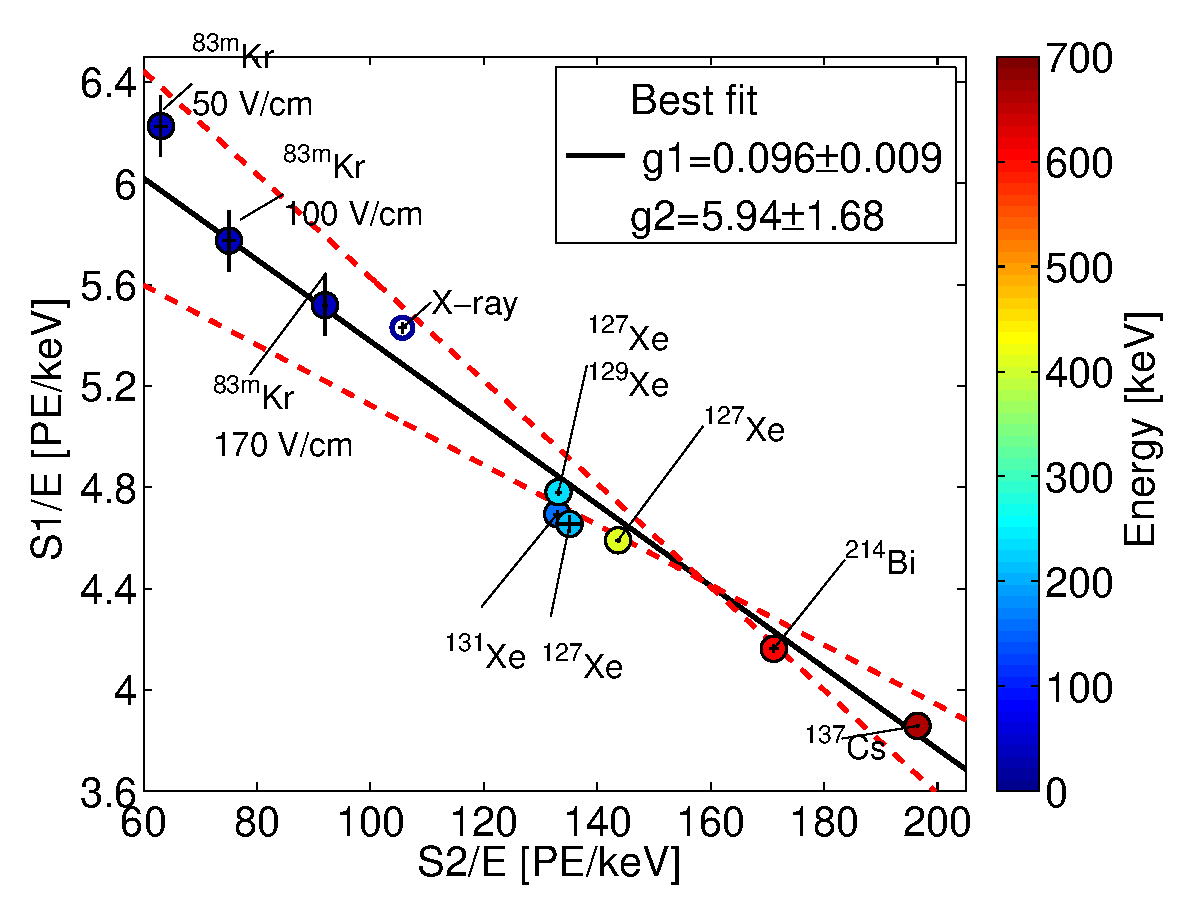
\includegraphics[width=130mm]{Chapter_E_Scale/Figures/Doke_new/S1S2_Doke_1.eps}
%\includegraphics[width=100mm]{Chapter_E_Scale/Figures/Doke_new/CD.png}
\caption{The Doke plot showing the mean values of S1/E vs S2/E for each calibration source. The data was cut by plotting the S2 vs the S1 and selecting the populations by eye, shown in figure \ref{fig:S1S2_space}. Using equation \ref {eq:g1g2_linfit}, the slope and intercept of the data constrain the parameters $\rm g_1$ and $\rm g_2$ The black solid line represent the best fit to the data and the red dashed lines represent $\pm 1\sigma$ of $\rm g_1$ and $\rm g_2$. The open circle is data from the K-shell xenon X-ray and was not used for the fit as its absolute energy and origin from the skin of the detector is uncertain.}
\label{fig:Doke1}
\end{figure}
\renewcommand{\baselinestretch}{2}
\small\normalsize
%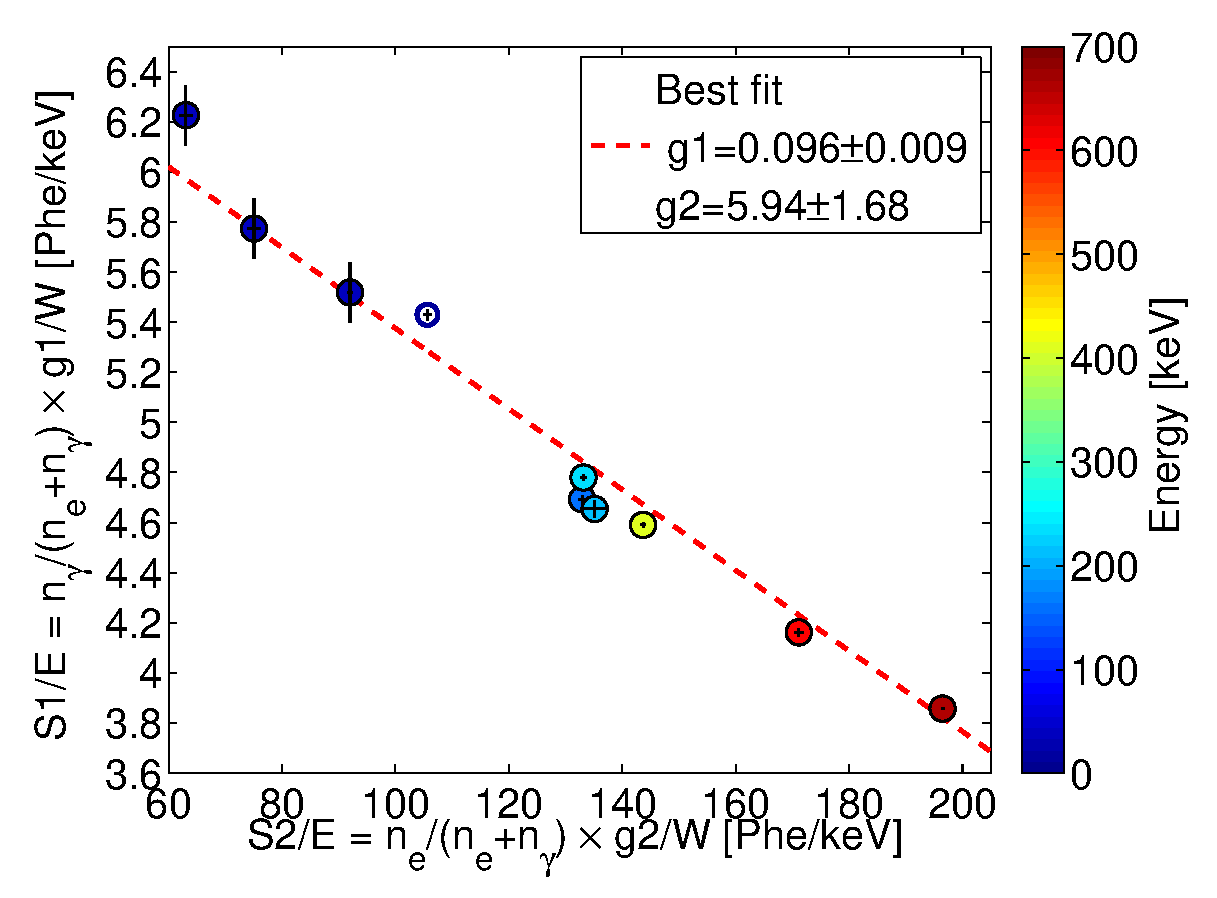
\includegraphics[width=120mm]{Chapter_E_Scale/Figures/S1S2_Doke_1.eps}
 
 \newpage
 
To better visualize the data on the Doke plot in figure \ref{fig:Doke1} all events from the calibration sources were added on the Doke plot, shown in figure \ref{fig:Doke1_Den}. The populations of the Xe activation lines and $\rm ^{214}Bi$ were isolated by the cuts shown in figure \ref{fig:S1S2_space}. By plotting in this way the populations of each source can be seen moving along a line of constant quanta (photons + electrons), which corresponds to the best fit for $\rm g_1$ and $\rm g_2$. The $\rm ^{137}Cs$ is moved along the line of constant quanta by recombination fluctuations and the \KrCal data is shifted as the different electric fields alter recombination probability. Note, recombination fluctuations will be discussed in section \ref{Ch:Flucs}. 

\renewcommand{\baselinestretch}{1}
\small\normalsize
 \begin{figure}[h!]\centering
%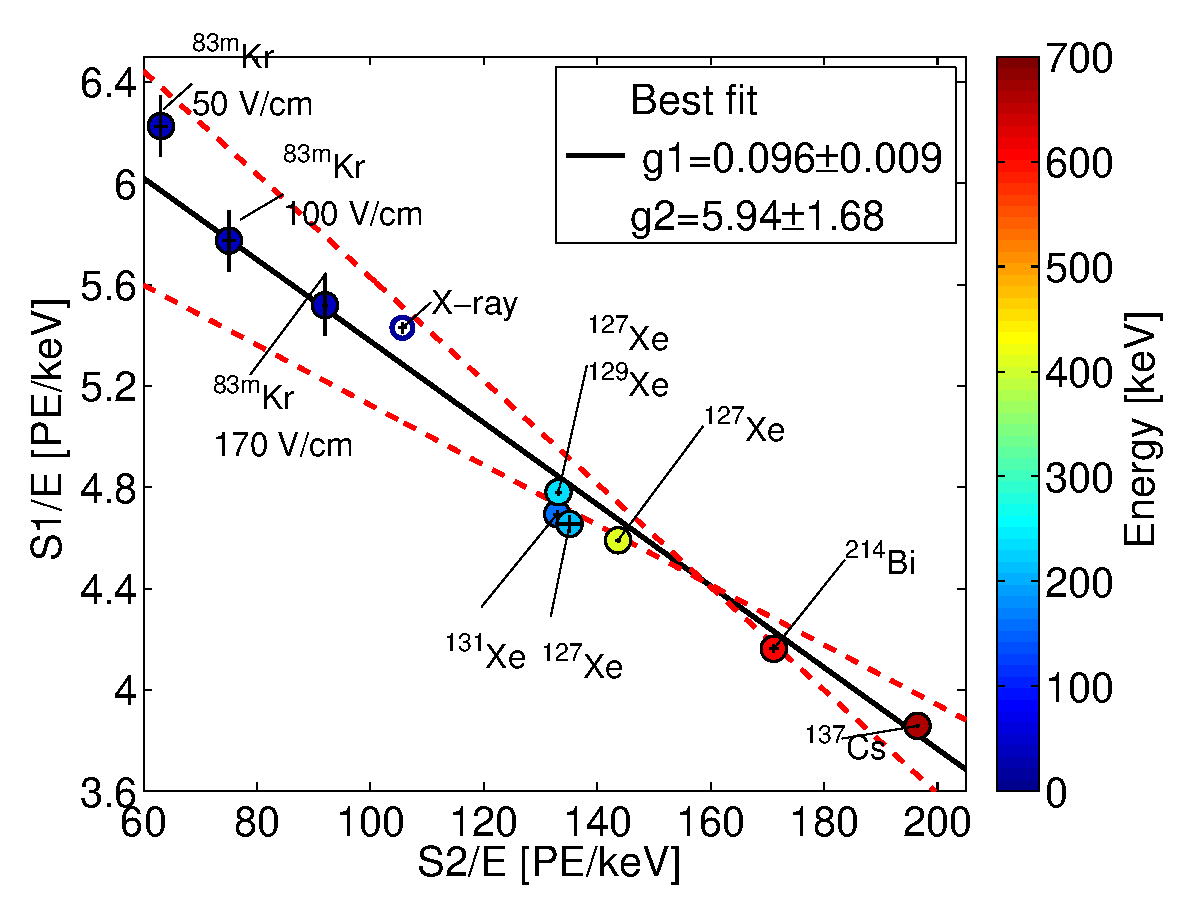
\includegraphics[width=130mm]{Chapter_E_Scale/Figures/Doke_new/S1S2_Doke_1.eps}
\includegraphics[width=130mm]{Chapter_E_Scale/Figures/Doke_new/CD.png}
\caption{Doke plot with all events from the calibration sources, with their S1 and S2 signal normalized to its corresponding energy. The populations of the Xe activation lines and $\rm ^{214}Bi$ were isolated by the cuts shown in figure \ref{fig:S1S2_space}. The solid black line represent the best fit to $\rm g_1$ and $\rm g_2$ and the dashed lines represents the 1 $\rm \sigma$ bounds.}
\label{fig:Doke1_Den}
\end{figure}
\renewcommand{\baselinestretch}{2}
\small\normalsize

\newpage

\section{Refitting in Combined Energy Space}
\label{sec:Doke2}
%From the first attempt to find $\rm g_1$ and $\rm g_2$ in figure \ref{fig:Doke1} there are discrepancies between the data and the fit, however 
This first result for $\rm g_1$ and $\rm g_2$, shown in figure \ref{fig:Doke1}, is only a crude estimate derived from isolating the populations in S1 vs. S2 space. Once we have an initial estimate of gains $\rm g_1$ and $\rm g_2$, a combined energy scale can be constructed with significantly improved resolution over the initial guess, due to the fact that recombination fluctuations are canceled. With the improved resolution the data are selected around their combined energy and fit using an un-binned maximum likelihood fit to a normal distribution. Then the data are refit around 1.5 $\sigma$ of the mean. The fits used to extract the means and sigmas  of the S1 and S2 signals at a given energy are shown in figures \ref{fig:Doke_Fits_S1} and \ref{fig:Doke_Fits_S2}. The energy spectra are shown later in figure \ref{fig:CE_hist}. The steps outlines are iterated twice as the convergence is rapid. In this case the initial value of $\rm g_1$ and $\rm g_2$ derived from cutting in S2 vs S1 space is already a close approximation to the true value. The resulting values of $\rm g_1$ and $\rm g_2$ are found to be 0.097$\pm$0.008 and 5.75$\pm$1.4 respectively. The fit is shown in figure \ref{fig:Doke2}. After refitting there is a significant improvement over figure \ref{fig:Doke1}, in terms of how well the data are described by the linear model of equation \ref {eq:g1g2_linfit}. This is especially notable for the the xenon activation lines in the center of the plot.  Note, the error on $\rm g_2$ is large relative to $\rm g_1$ due to the greater separation of the calibration pints from the x intercept. 

%\begin{equation}
%\begin{split}
%\rm  g_1 = 0.097\pm0.008 \\
%\rm  g_2= 5.75\pm1.4
%\label{eq:g1g2Fit}
%\end{split}
%\end{equation}

\renewcommand{\baselinestretch}{1}
\small\normalsize
 \begin{figure}[h!]\centering
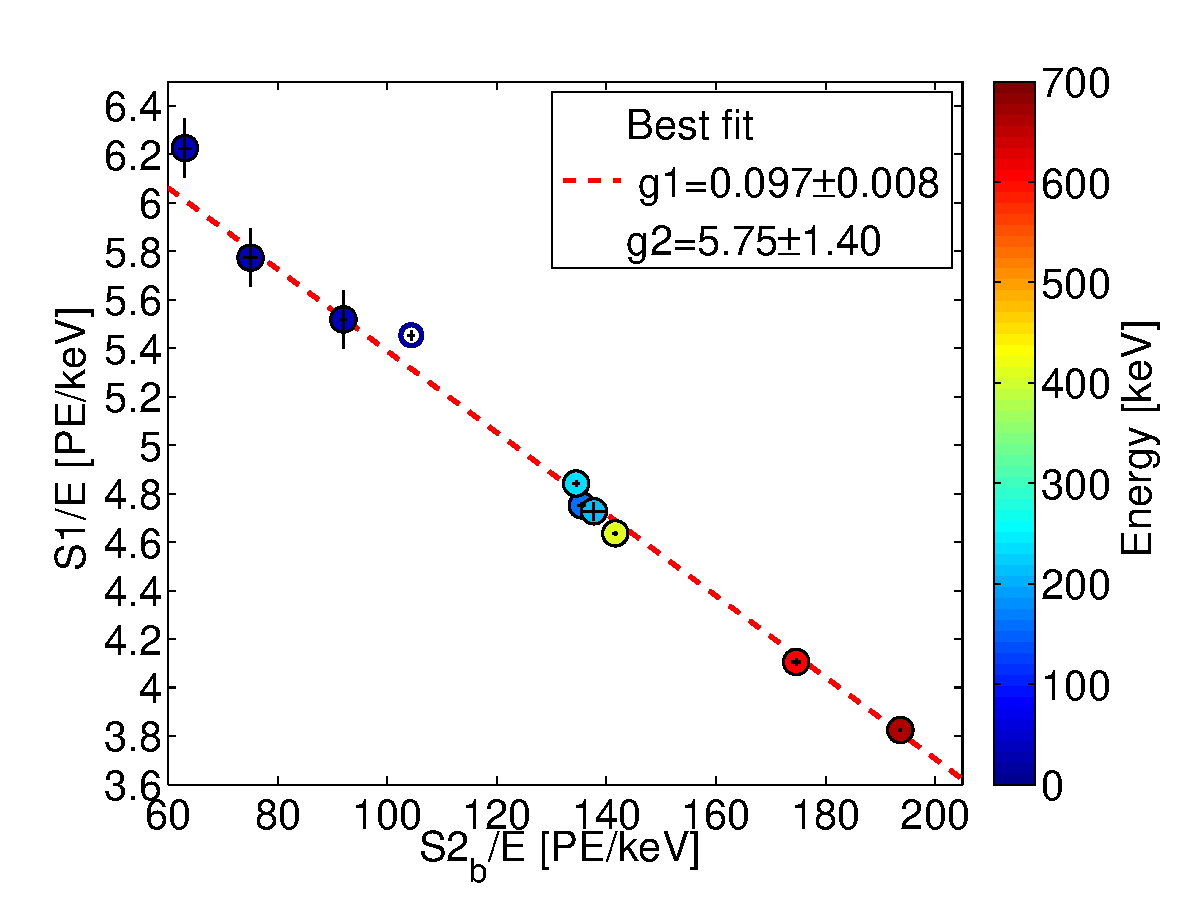
\includegraphics[width=130mm]{Chapter_E_Scale/Figures/Doke_new/S1S2_Doke_3.eps}
\caption{The Doke plot showing the mean values of S1/E vs S2/E for each calibration source. The data has been further cut upon the combined energy reconstructed from an initial best fit to the data. Using equation \ref{eq:g1g2_linfit}, the slope and intercept of the data constrain the parameters $\rm g_1$ and $\rm g_2$ The black solid line represent the best fit to the data and the red dashed lines represent $\pm 1\sigma$ of $\rm g_1$ and $\rm g_2$. The open circle is data from the K-shell xenon X-ray and was not used for the fit as its absolute energy and origin from the skin of the detector is uncertain.}
\label{fig:Doke2}
\end{figure}
\renewcommand{\baselinestretch}{2}
\small\normalsize

 \begin{figure}[h!]\centering
 
\subcaptionbox{\label{fig:1a}}{\includegraphics[width=45mm]{Chapter_E_Scale/Figures/Doke_Fits_2/fit_S1_163.eps}}
\hfill
\subcaptionbox{\label{fig:1b}}{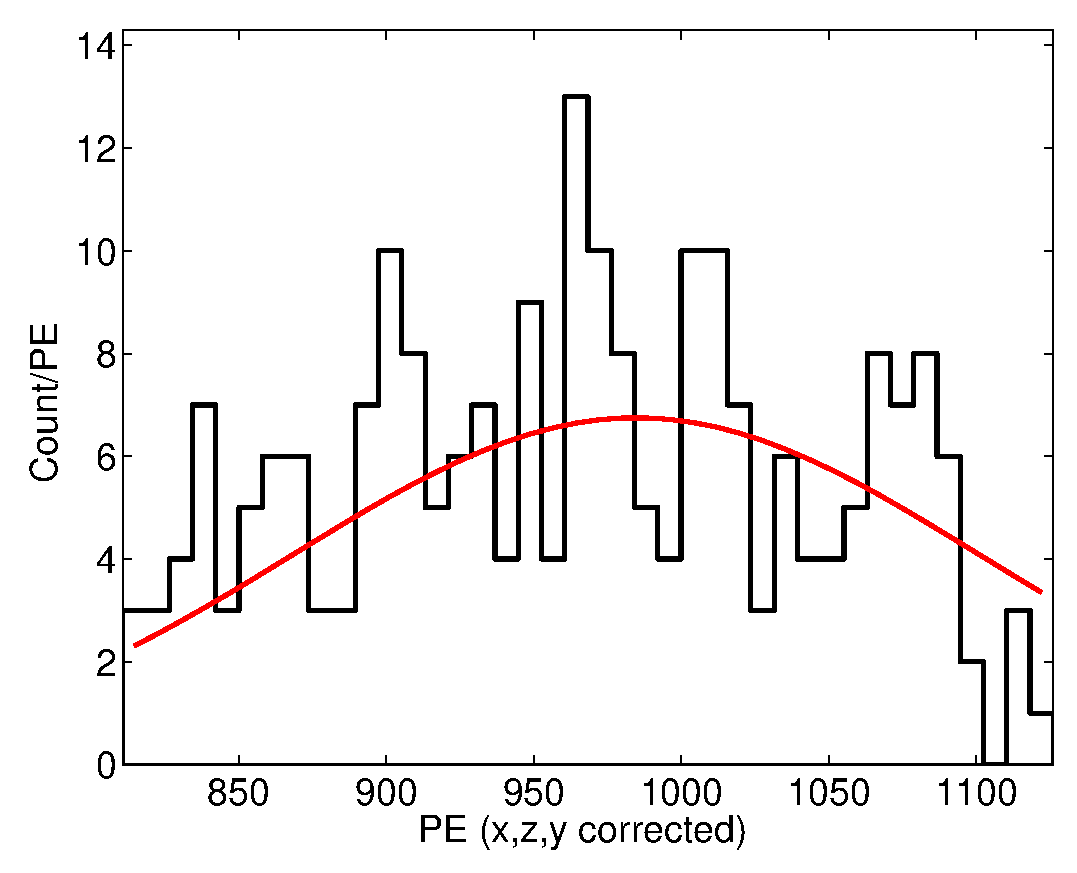
\includegraphics[width=45mm]{Chapter_E_Scale/Figures/Doke_Fits_2/fit_S1_207.eps}}
\hfill
\subcaptionbox{\label{fig:1c}}{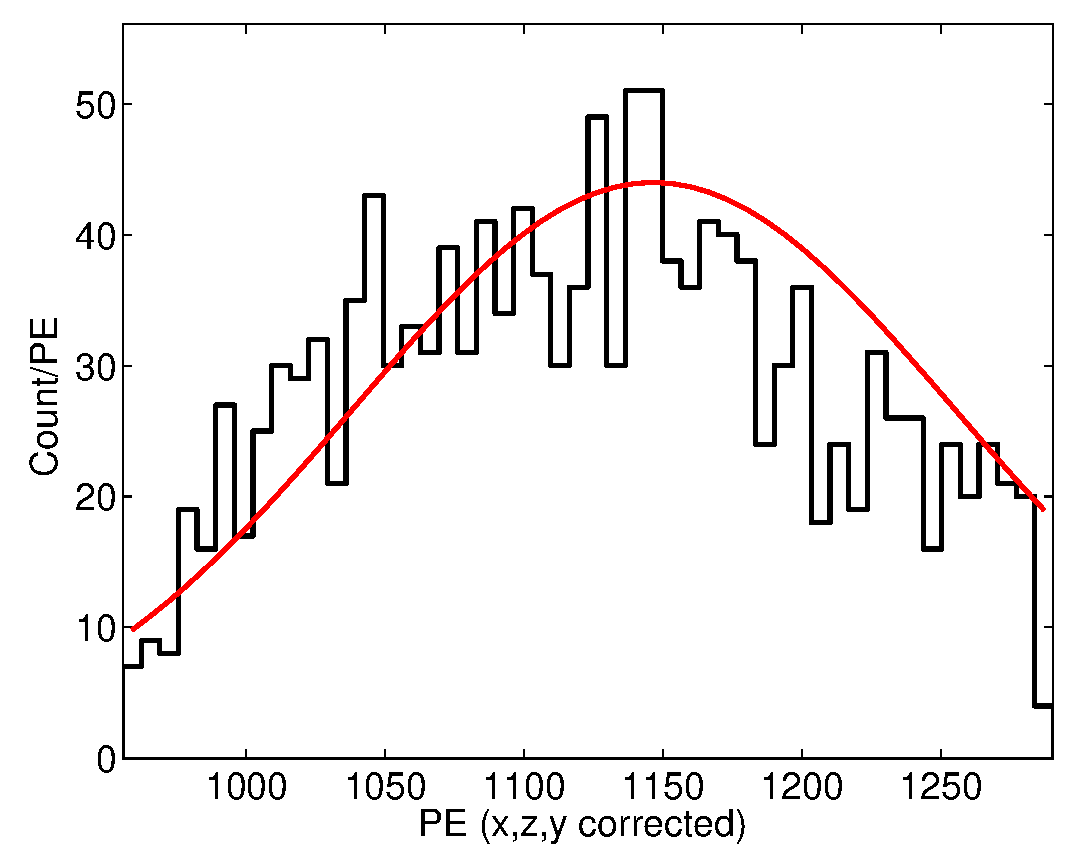
\includegraphics[width=45mm]{Chapter_E_Scale/Figures/Doke_Fits_2/fit_S1_236.eps}}

\bigskip

\subcaptionbox{\label{fig:1d}}{\includegraphics[width=45mm]{Chapter_E_Scale/Figures/Doke_Fits_2/fit_S1_410.eps}}
\hfill
\subcaptionbox{\label{fig:1e}}{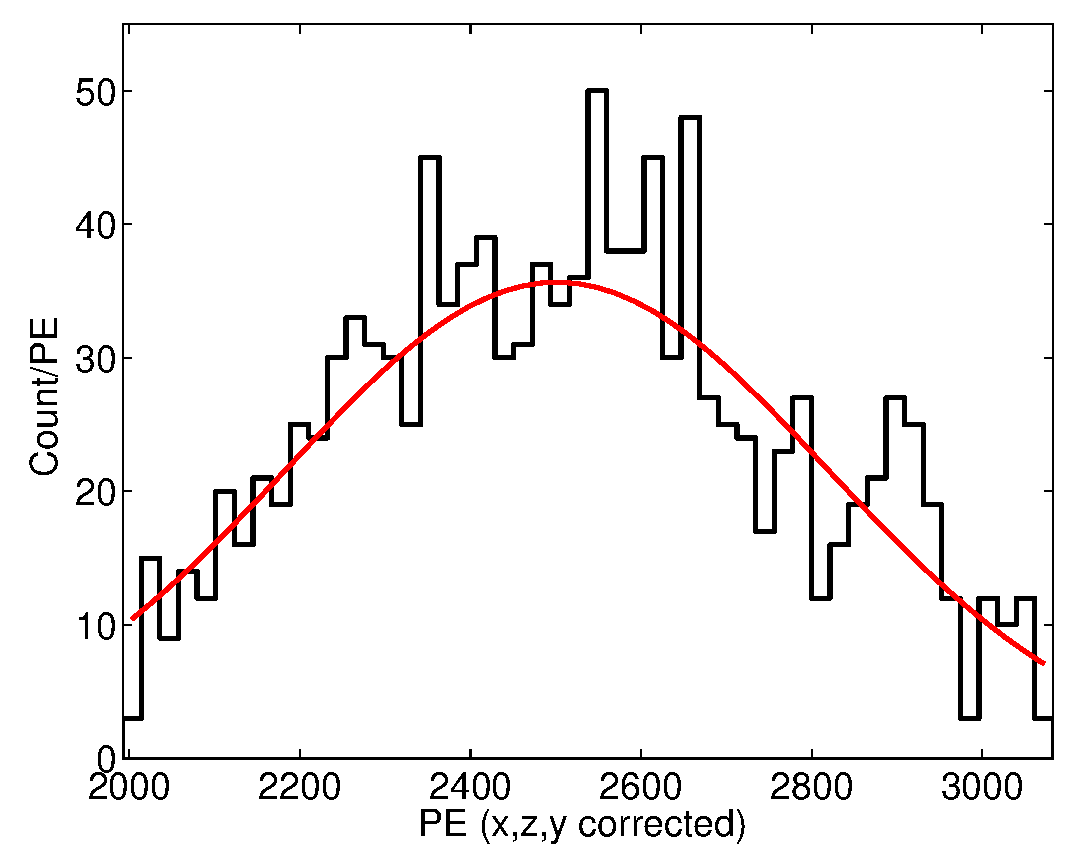
\includegraphics[width=45mm]{Chapter_E_Scale/Figures/Doke_Fits_2/fit_S1_Bi214.eps}}
\hfill
\subcaptionbox{\label{fig:1f}}{\includegraphics[width=45mm]{Chapter_E_Scale/Figures/Doke_Fits_2/fit_S1_Cs137.eps}}

\bigskip

\subcaptionbox{\label{fig:1g}}{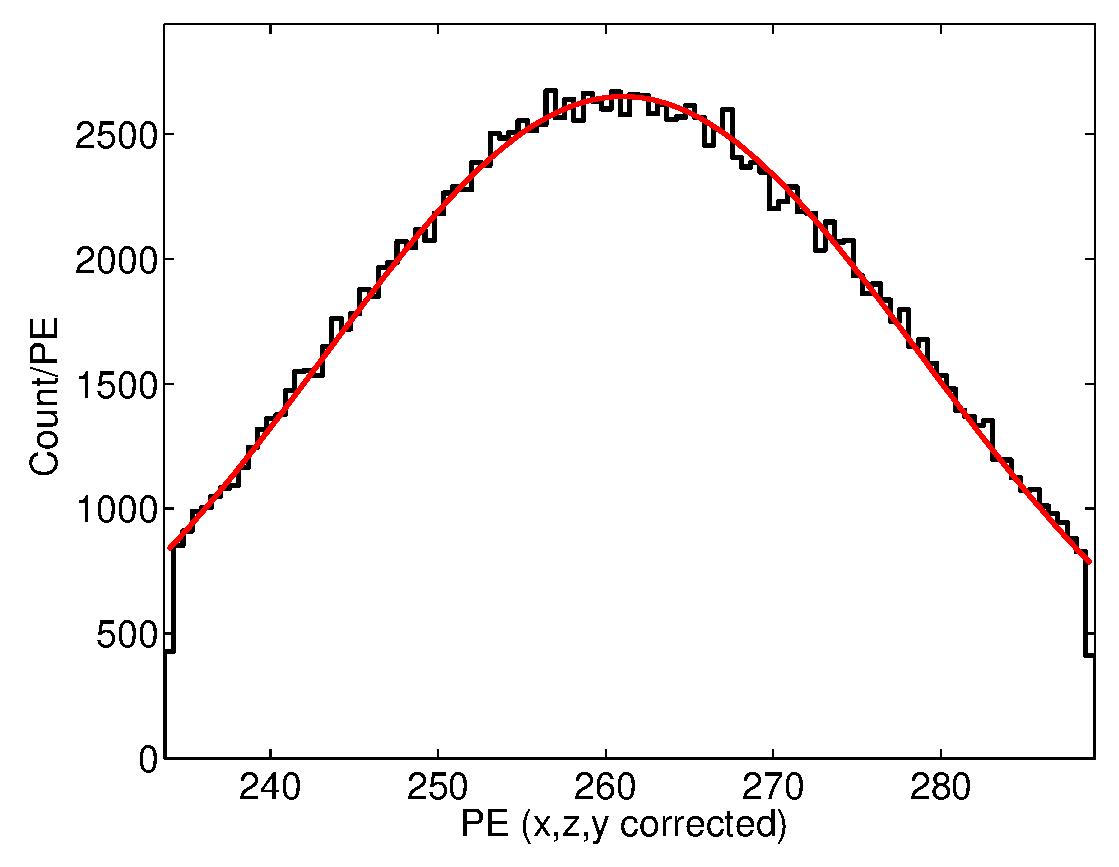
\includegraphics[width=45mm]{Chapter_E_Scale/Figures/Doke_Fits_2/fit_S1_Kr_50.eps}}
\hfill
\subcaptionbox{\label{fig:1h}}{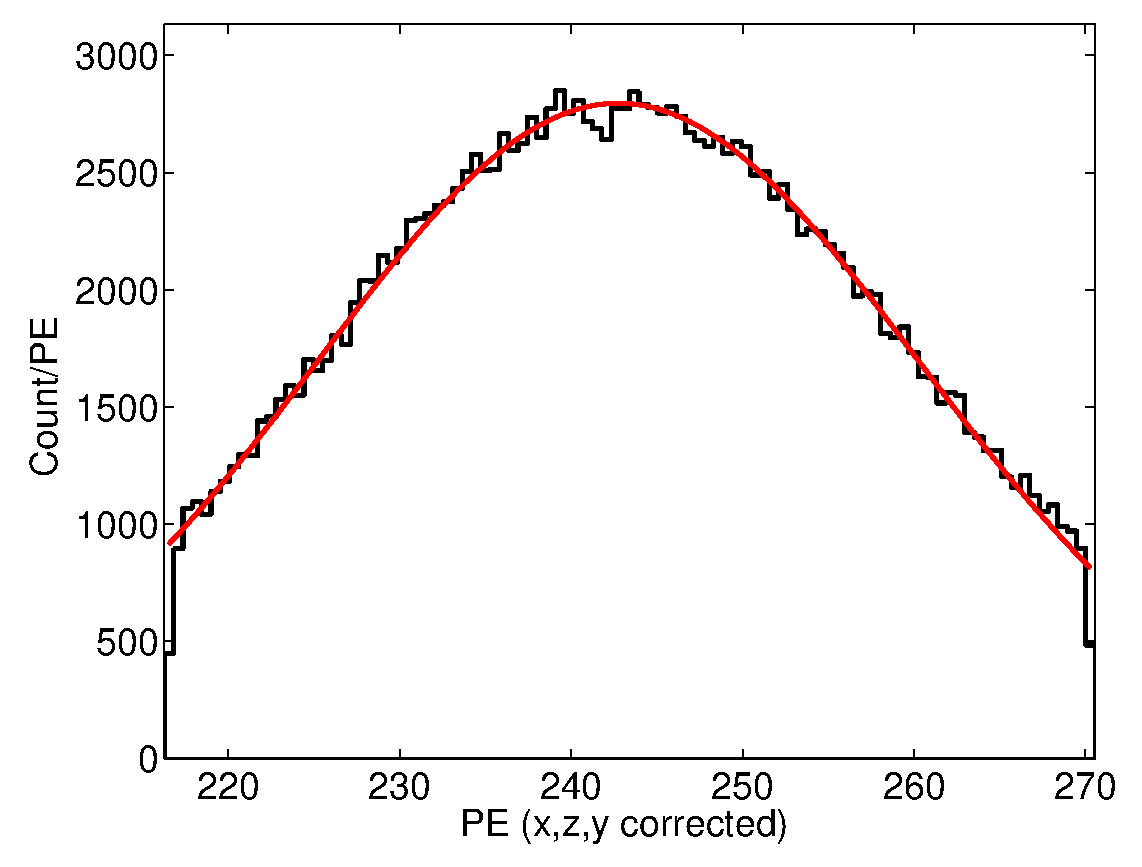
\includegraphics[width=45mm]{Chapter_E_Scale/Figures/Doke_Fits_2/fit_S1_Kr_100.eps}}
\hfill
\subcaptionbox{\label{fig:1i}}{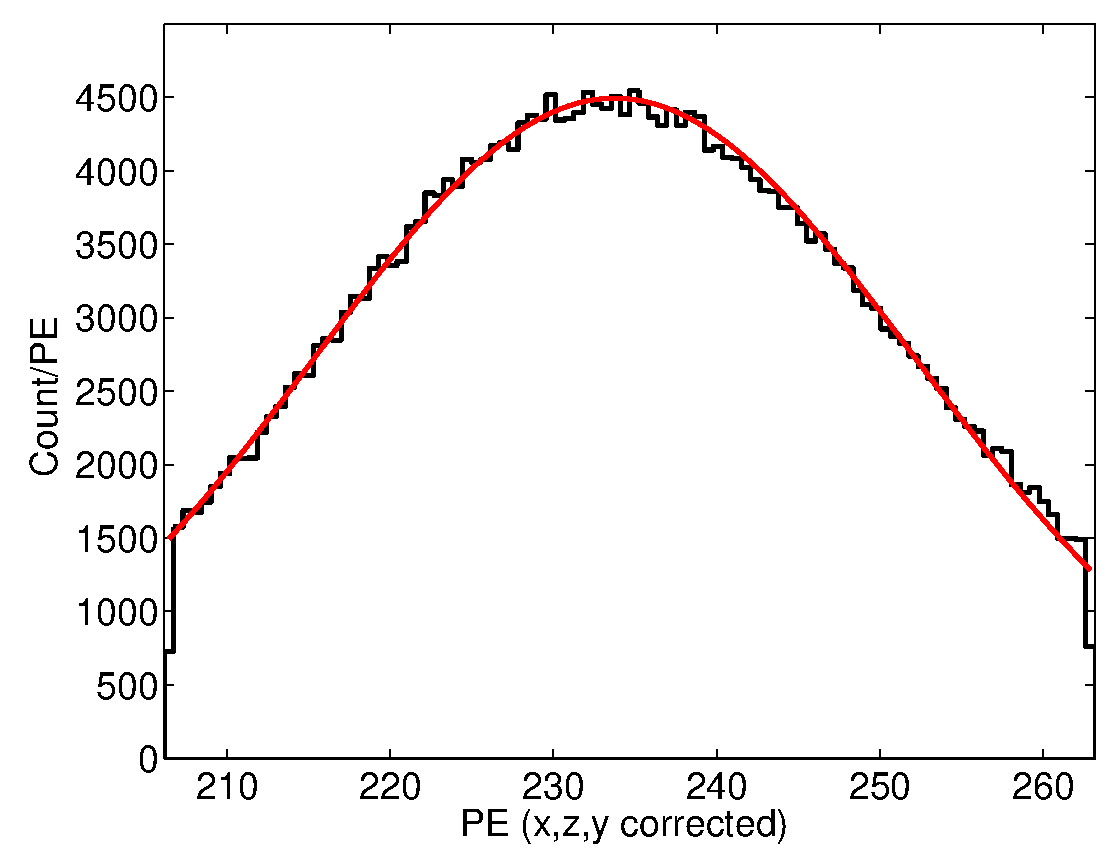
\includegraphics[width=45mm]{Chapter_E_Scale/Figures/Doke_Fits_2/fit_S1_Kr.eps}}

\caption{S1 fits to sources at nominal field of 170 V/cm unless otherwise noted. Source and energy in keV from top left to bottom right: a) $\rm ^{131}Xe$: 163, b) $\rm ^{127}Xe$:  207, c) $\rm ^{127}Xe$ \&  $\rm ^{129m}Xe$: 236.8, d)  $\rm ^{127}Xe$: 410, e) $\rm ^{214}Bi$: 609, f) $\rm ^{137}Cs$: 661.6, g) $\rm ^{83m}Kr$: 41.5 - at 50 V/cm, h) $\rm ^{83m}Kr$ 41.5 - at 100 V/cm, i) $\rm ^{83m}Kr$ 41.5 .}
\label{fig:Doke_Fits_S1}
\end{figure}


 \begin{figure}[h!]\centering
 
\subcaptionbox{\label{fig:1a}}{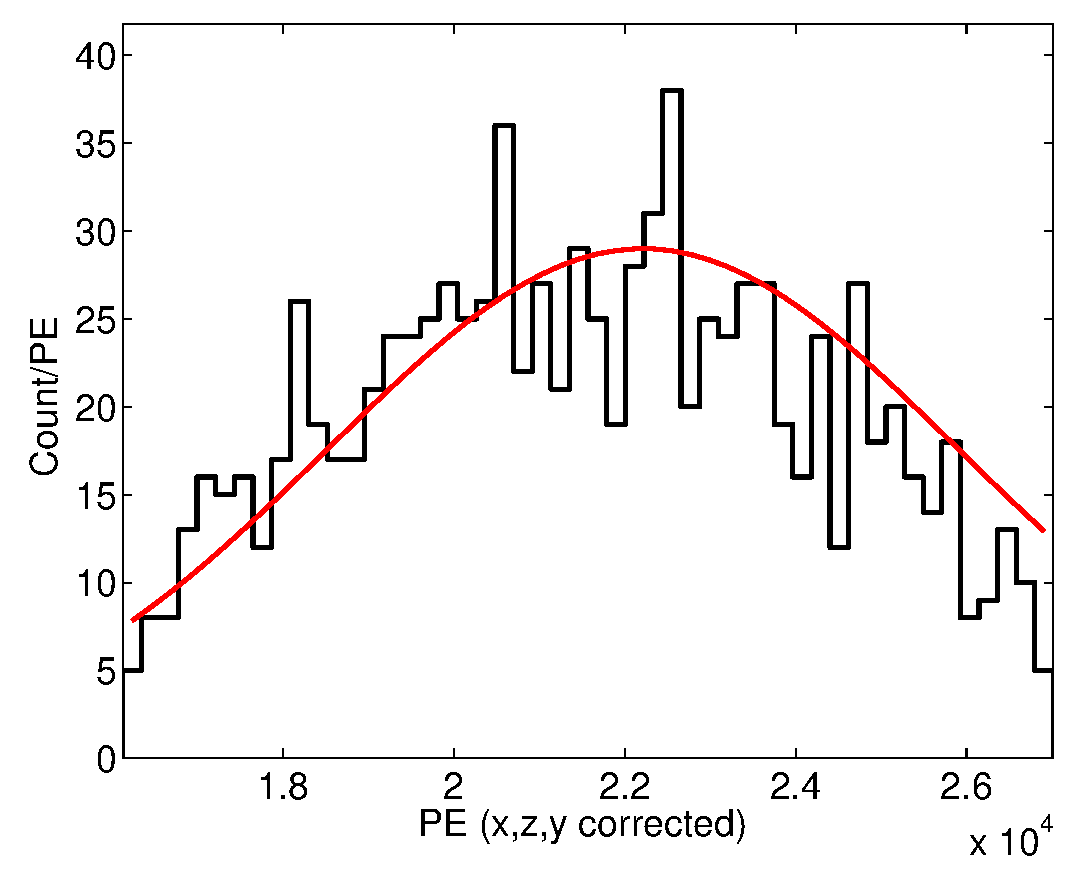
\includegraphics[width=45mm]{Chapter_E_Scale/Figures/Doke_Fits_2/fit_S2_163.eps}}
\hfill
\subcaptionbox{\label{fig:1b}}{\includegraphics[width=45mm]{Chapter_E_Scale/Figures/Doke_Fits_2/fit_S2_207.eps}}
\hfill
\subcaptionbox{\label{fig:1c}}{\includegraphics[width=45mm]{Chapter_E_Scale/Figures/Doke_Fits_2/fit_S2_236.eps}}

\bigskip

\subcaptionbox{\label{fig:1d}}{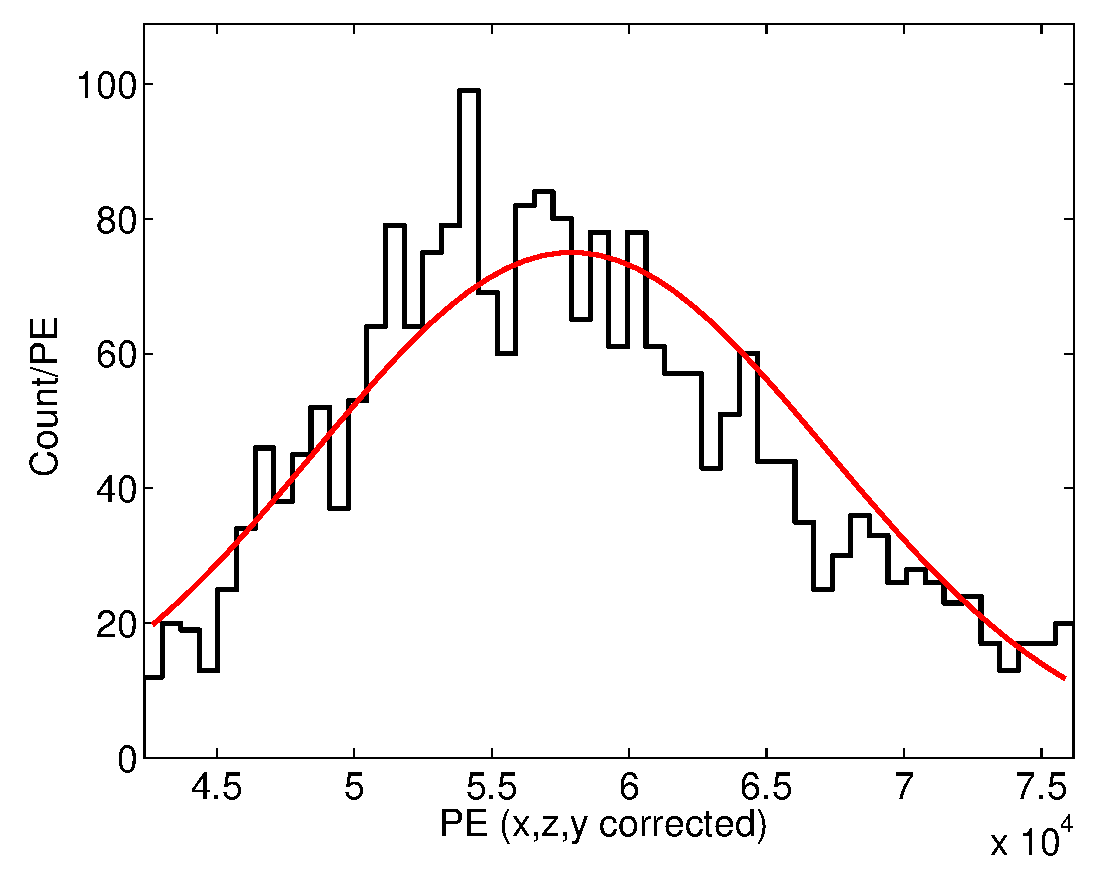
\includegraphics[width=45mm]{Chapter_E_Scale/Figures/Doke_Fits_2/fit_S2_410.eps}}
\hfill
\subcaptionbox{\label{fig:1e}}{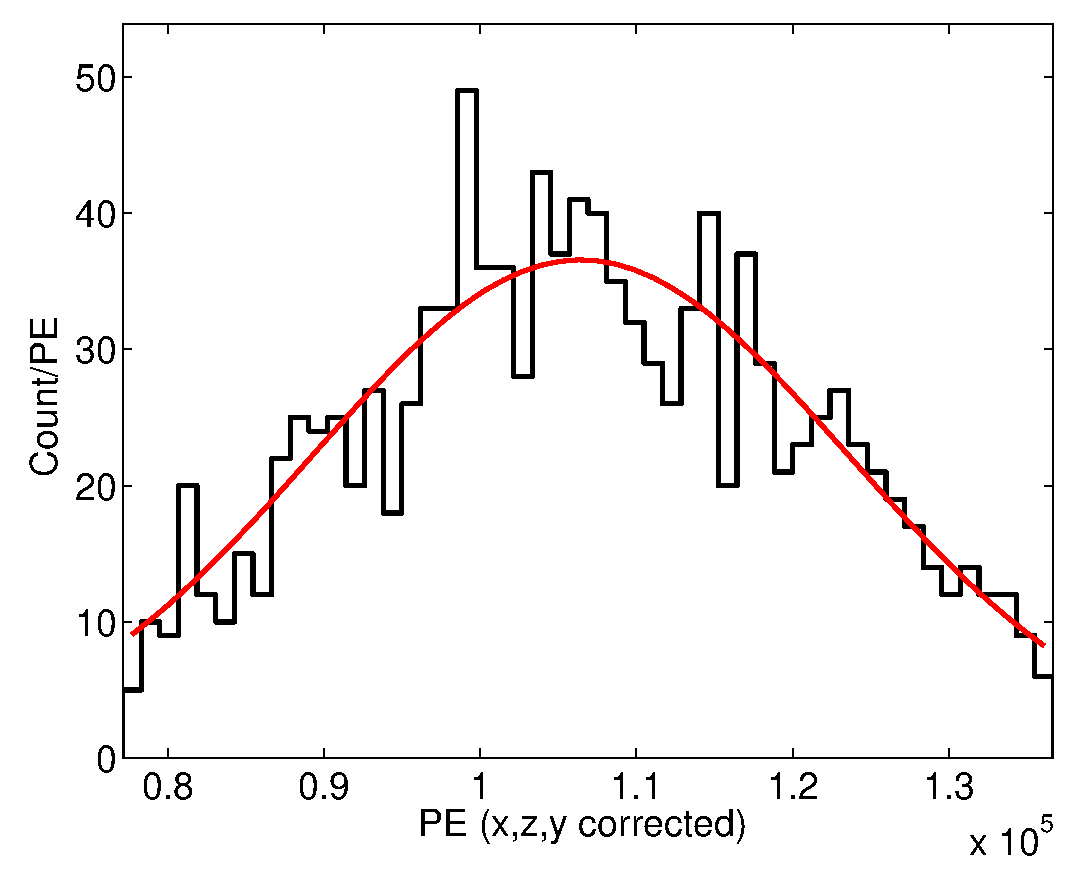
\includegraphics[width=45mm]{Chapter_E_Scale/Figures/Doke_Fits_2/fit_S2_Bi214.eps}}
\hfill
\subcaptionbox{\label{fig:1f}}{\includegraphics[width=45mm]{Chapter_E_Scale/Figures/Doke_Fits_2/fit_S2_Cs137.eps}}

\bigskip

\subcaptionbox{\label{fig:1g}}{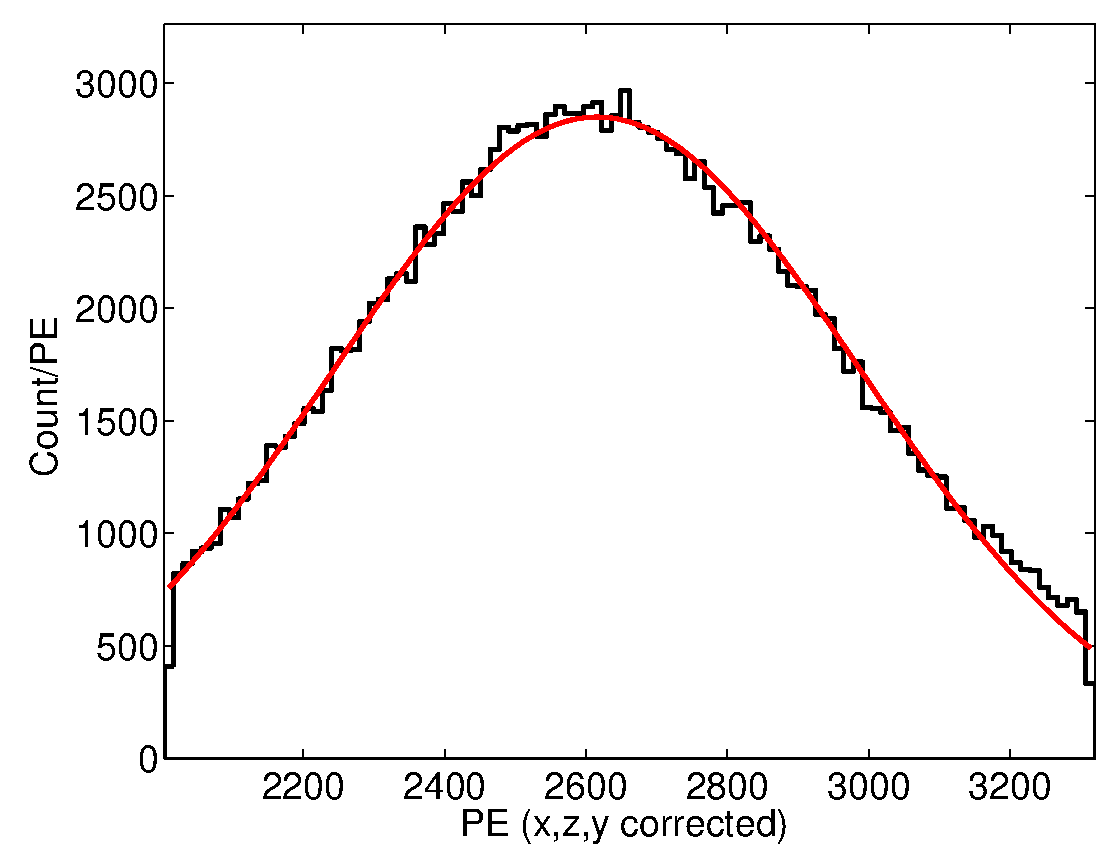
\includegraphics[width=45mm]{Chapter_E_Scale/Figures/Doke_Fits_2/fit_S2_Kr_50.eps}}
\hfill
\subcaptionbox{\label{fig:1h}}{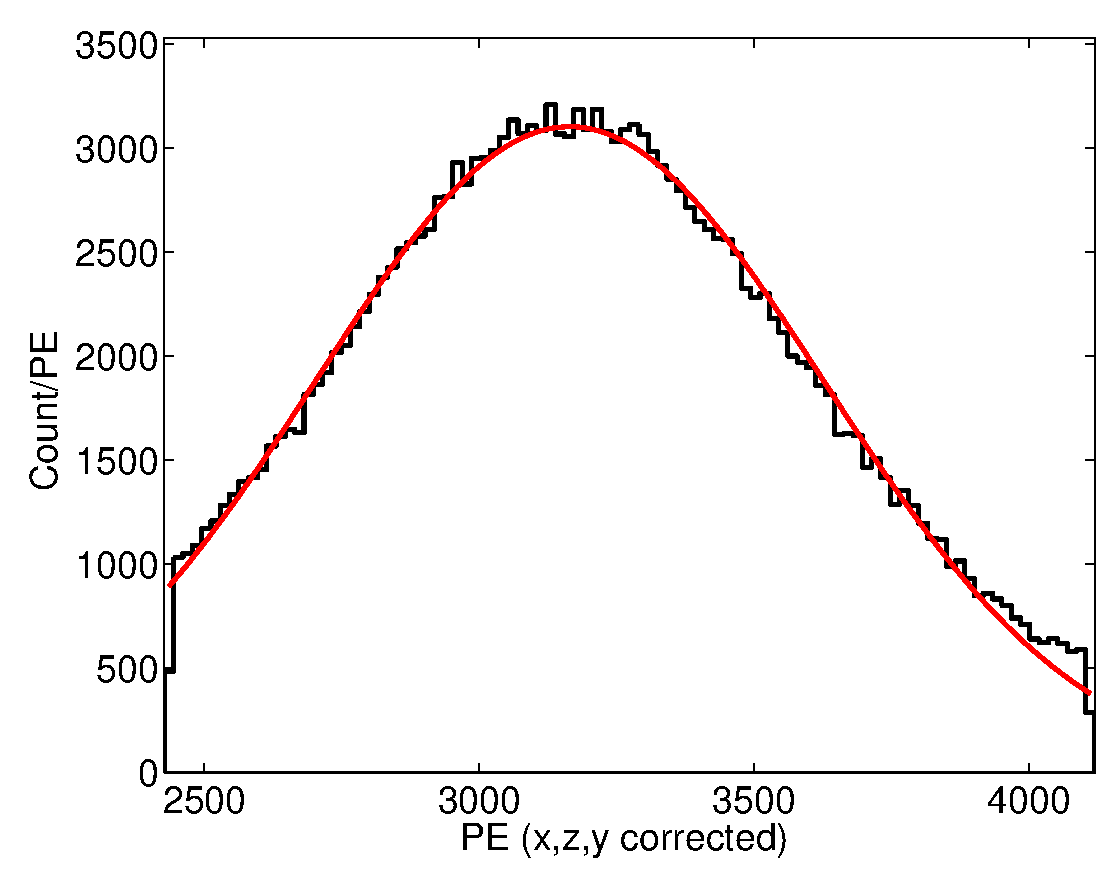
\includegraphics[width=45mm]{Chapter_E_Scale/Figures/Doke_Fits_2/fit_S2_Kr_100.eps}}
\hfill
\subcaptionbox{\label{fig:1i}}{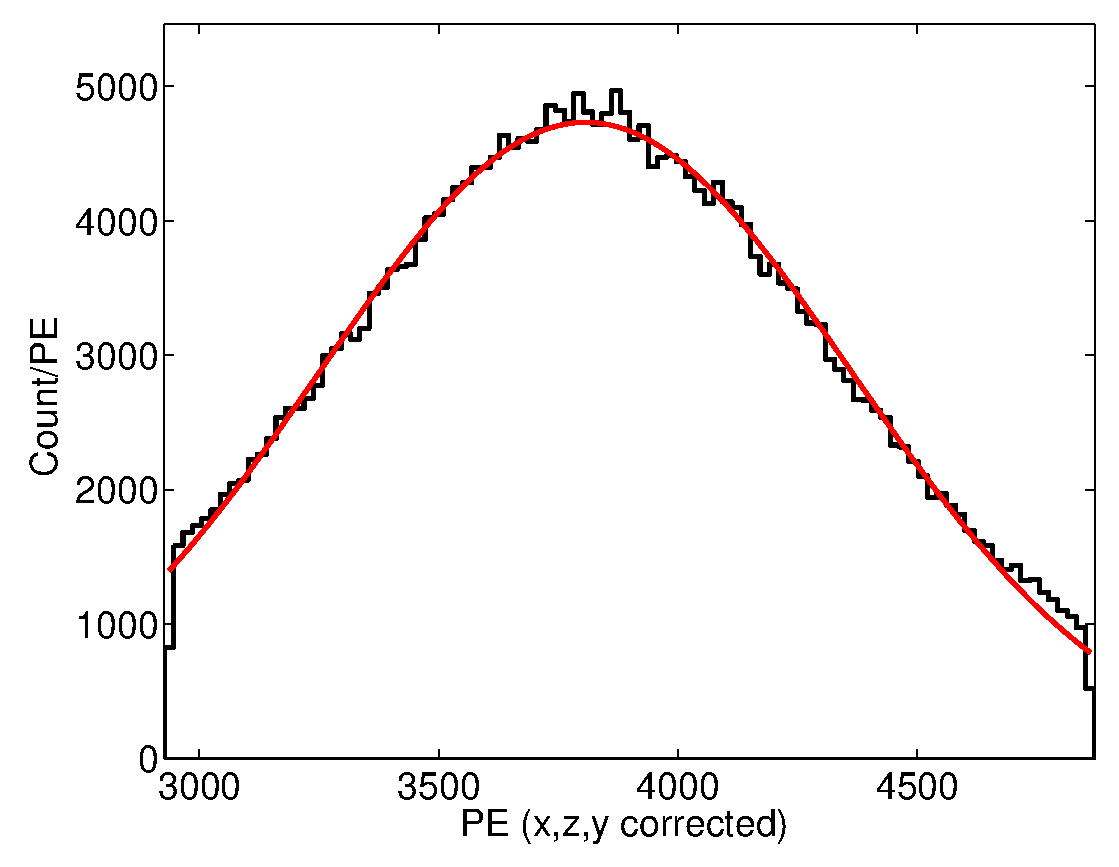
\includegraphics[width=45mm]{Chapter_E_Scale/Figures/Doke_Fits_2/fit_S2_Kr.eps}}

\caption{S2 fits to sources at nominal field of 170 V/cm unless otherwise noted. Source and energy in keV from top left to bottom right: a) $\rm ^{131}Xe$: 163, b) $\rm ^{127}Xe$:  207, c) $\rm ^{127}Xe$ \&  $\rm ^{129m}Xe$: 236.8, d)  $\rm ^{127}Xe$: 410, e) $\rm ^{214}Bi$: 609, f) $\rm ^{137}Cs$: 661.6, g) $\rm ^{83m}Kr$: 41.5 - at 50 V/cm, h) $\rm ^{83m}Kr$ 41.5 - at 100 V/cm, i) $\rm ^{83m}Kr$ 41.5 .}
\label{fig:Doke_Fits_S2}
\end{figure}


Figure \ref{fig:Doke_E} shows another representation of the idea behind equation \ref{eq:g1g2_linfit}. The combined energy model describes the data well using the optimal fit for $\rm g_1$ and $\rm g_2$. For each increase in number of photons there is a corresponding equal decrease in the number of electrons and visa-versa. As stated before the values of $\rm g_1$ and $\rm g_2$ are highly anti-correlated because the data, relatively far from the x and y intercepts, constrains their ratio only. Thus, for future studies it will be important to probe more of the charge vs light parameter space in order to place a tighter constraint on gains $\rm g_1$ and $\rm g_2$. This can be achieved by both modifying the electric field inside the detector and by using more calibration sources.


 \begin{figure}[h!]\centering
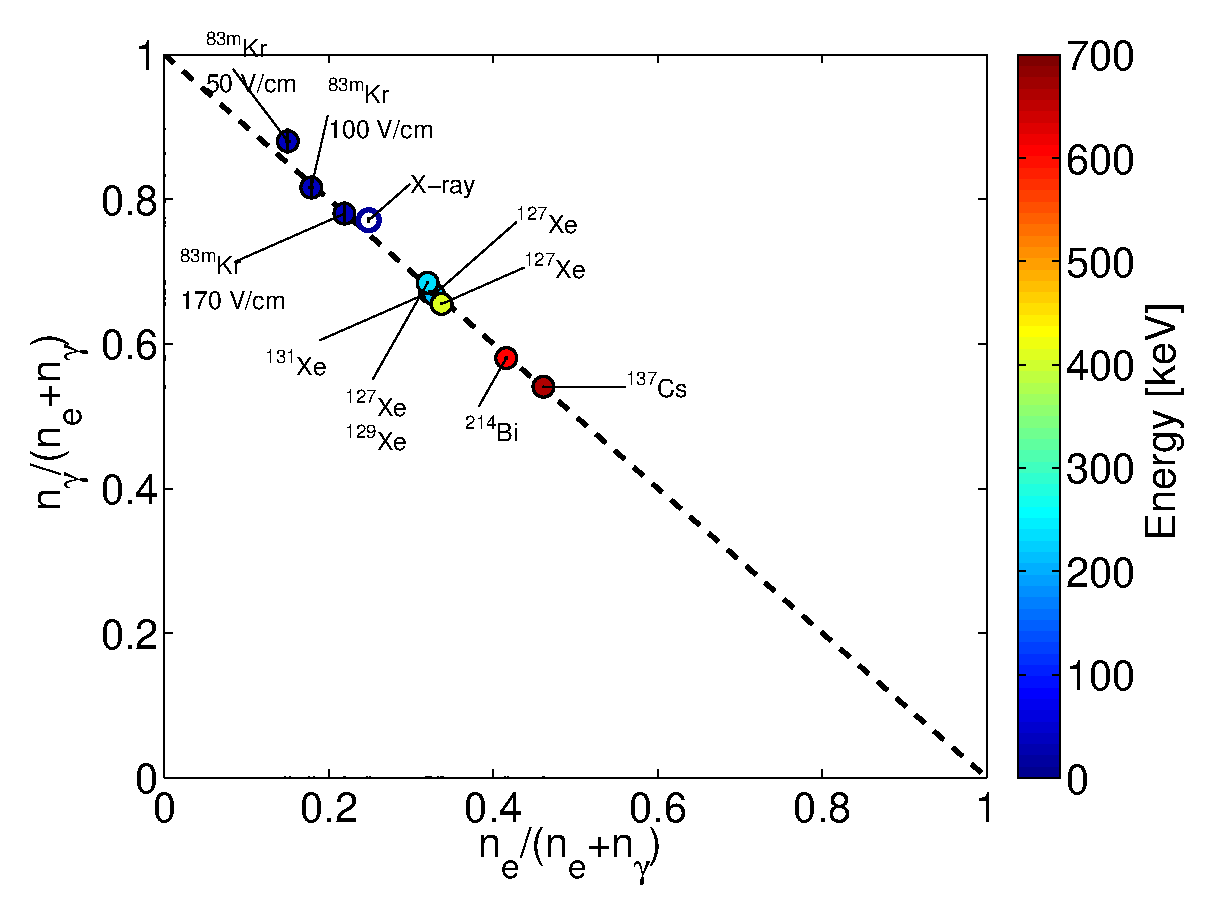
\includegraphics[width=130mm]{Chapter_E_Scale/Figures/Doke_new/S1S2_Doke2_3.eps}
\caption{Doke plot of the data showing the light yield vs. charge yield. In this version of the plot, S2/E has been scaled by W/$\rm g_2$ so that the x-axis corresponds to the ratio of $\rm n_e$ to total quanta. Similarly S1/E has been scaled by W/$\rm g_1$ so that the y axis corresponds to the ratio of $\rm n_\gamma$ to total quanta. The black horizontal line represents moving along the line of constant quanta, for each additional photon an electron is lost as visa-vera.}
\label{fig:Doke_E}
\end{figure}

\newpage

\section{Error Determination of $\rm g_1$ and $\rm g_2$ with a Markov Chain Monte Carlo}
\label{sec:MCMC}
The error bars reported in sections \ref{sec:Doke1} and \ref{sec:Doke1} on $\rm g_1$ and $\rm g_2$ are from the error in the slope and intercept of the linear fit in the Doke plot and are derived using a MCMC (Markov Chain Monte Carlo). For calculating the error in slope and intercept  three random walkers were used at each data point and allowed to take 500 steps.The MCMC takes into account the covariance of the parameters, shown in figure \ref{fig:MCMC} as a two dimensional Gaussian. There is a strong negative correlation between the slope m and intercept b which is the result of the degeneracy between gains $\rm g_1$ and $\rm g_2$ Thus, the error on $\rm g_1$ and $\rm g_2$ is such that for the positive maxima deviation in $\rm g_1$ we reach the negative maxima of the error on $\rm g_2$, and visa-versa.


\begin{figure}[h!]\centering
\includegraphics[width=100mm]{Chapter_E_Scale/Figures/MCMC/triangle.png} % also line-time.png
\caption{MCMC for the linear fit to the Doke plot. There is a strong negative correlation between the slope m and intercept b which results from the degeneracy between gains $\rm g_1$ and $\rm g_2$. }
\label{fig:MCMC} 
\end{figure}

\newpage

\section{Combined Energy Space}

With the values of $\rm g_1$ and $\rm g_2$ known the combined energy of events can be reconstructed with a significant improvement over using only the light or charge channel. In combined energy space recombination fluctuations are removed by the anti correlation of light and charge production and any residual smearing is due to intrinsic detector resolution (discussed later in section \ref{Ch:Flucs}) . Figure \ref{fig:CE_hist} shows the energy histograms of the data used for the fits to gains $\rm g_1$ and $\rm g_2$ including the xenon activation lines and the $\rm^{137}Cs$ calibration, along with a zoom-in of the xenon K shell Xray around 29-34 keV. 


\begin{figure}[h!]\centering
 
\subcaptionbox{\label{fig:1a}}{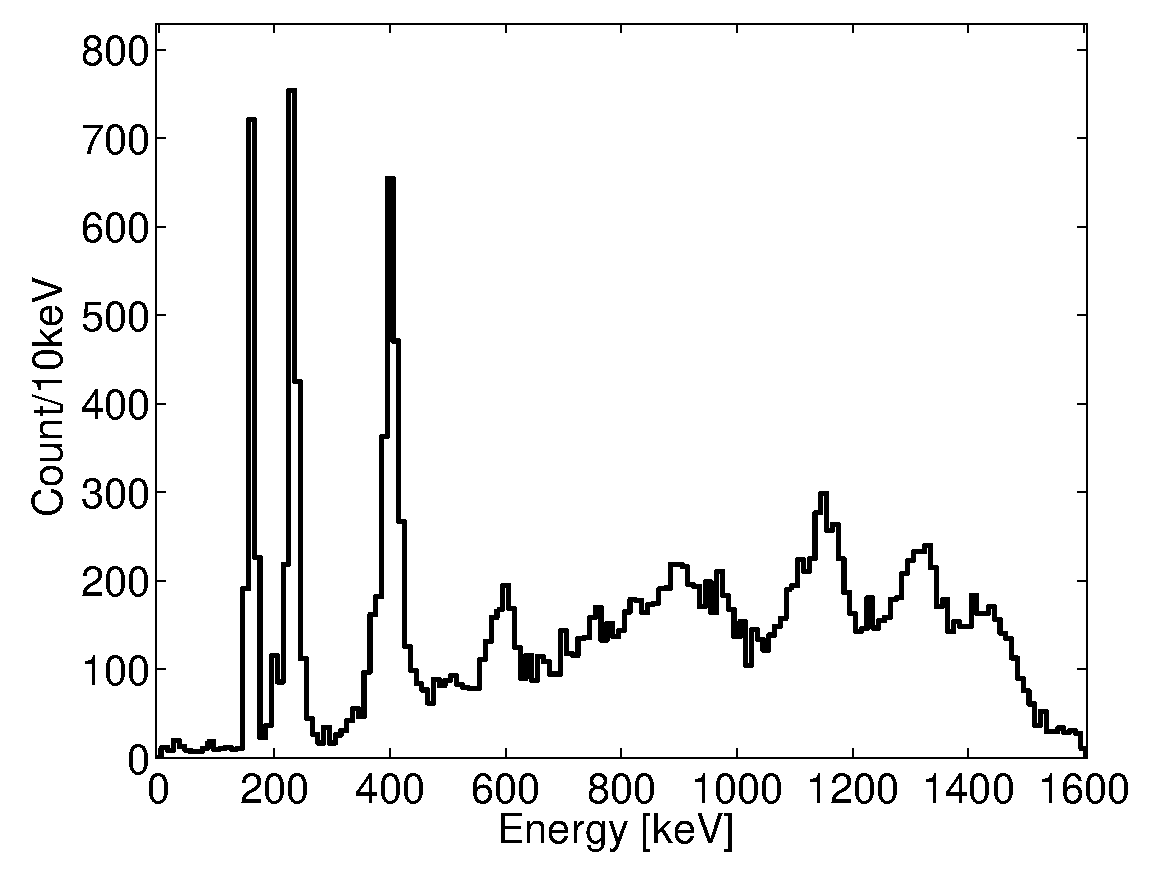
\includegraphics[width=70mm]{Chapter_E_Scale/Figures/Combined_E/Xe_act_E.eps}}
\hfill
\subcaptionbox{\label{fig:1b}}{\includegraphics[width=70mm]{Chapter_E_Scale/Figures/Combined_E/Cs_E.eps}}


\bigskip

\subcaptionbox{\label{fig:1c}}{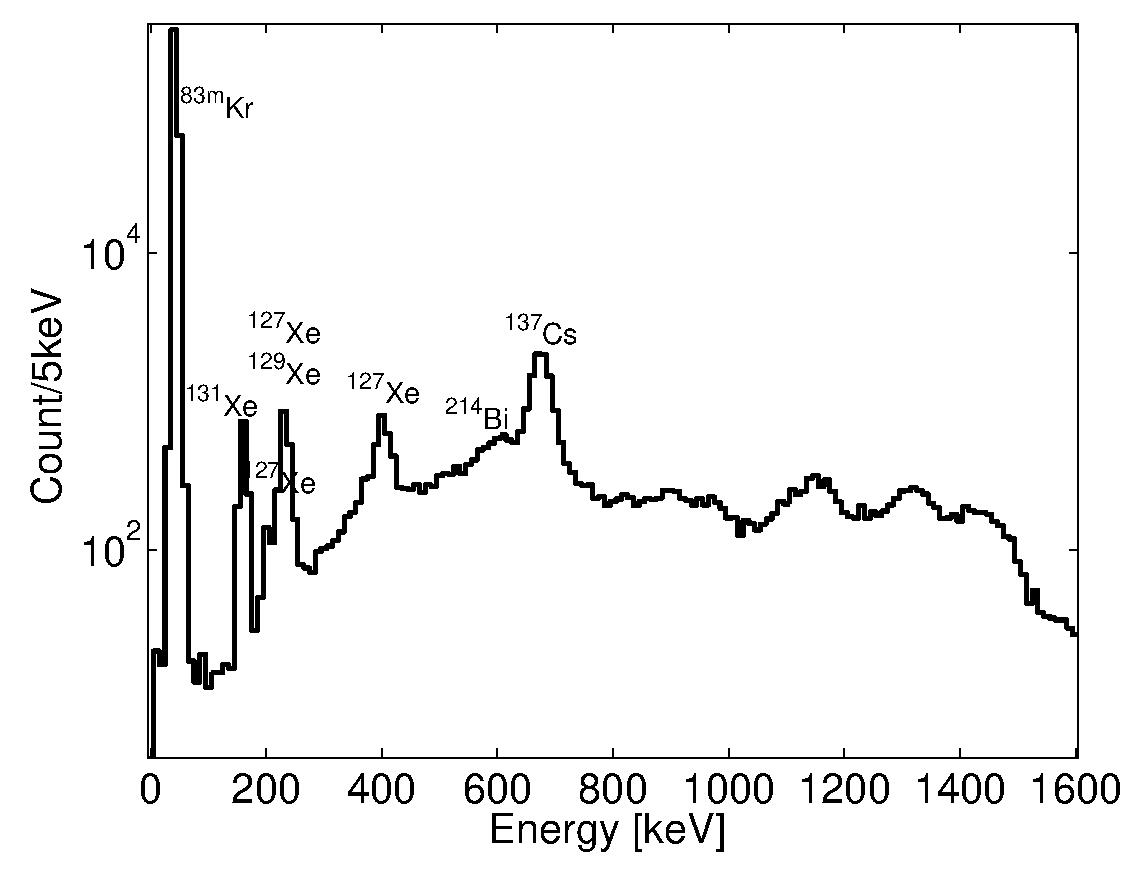
\includegraphics[width=70mm]{Chapter_E_Scale/Figures/Combined_E/Cs_Kr_Xe_E.eps}}
\hfill
\subcaptionbox{\label{fig:1d}}{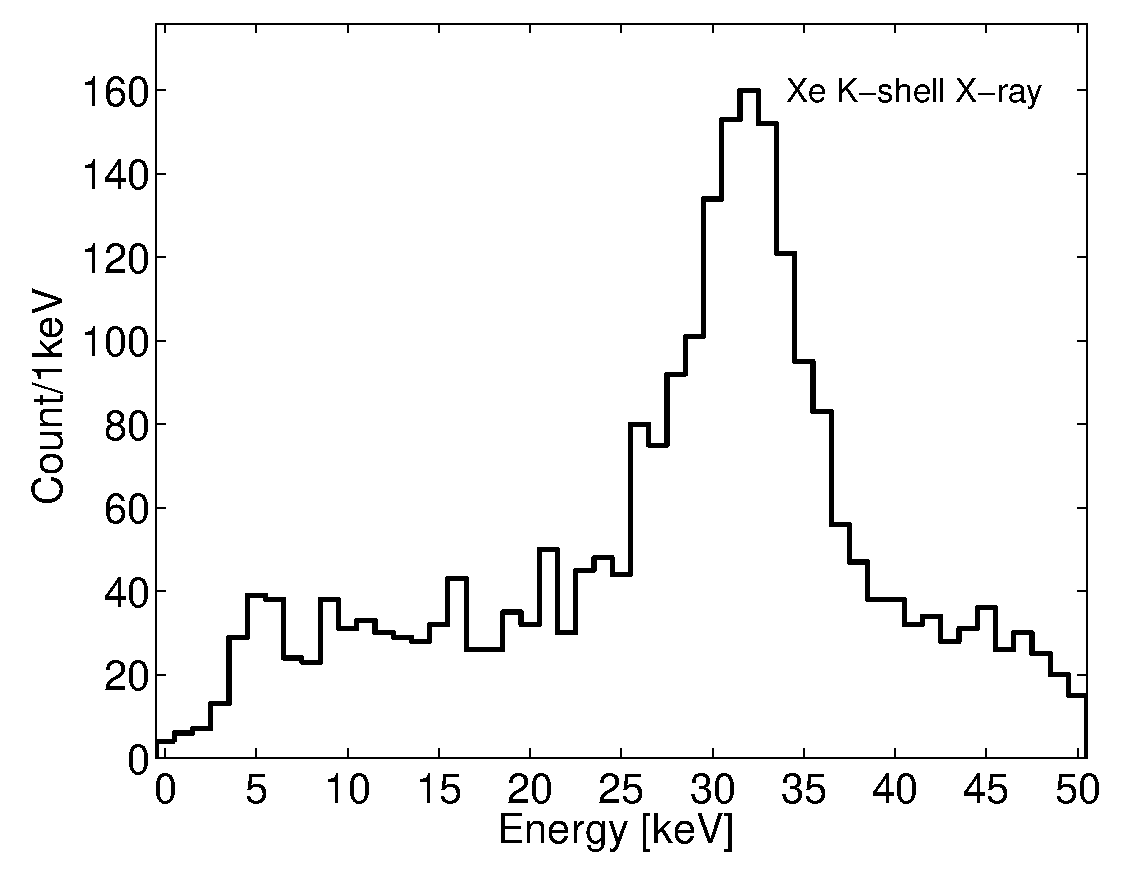
\includegraphics[width=70mm]{Chapter_E_Scale/Figures/Combined_E/X-ray_Xe_E.eps}}


\caption{Combined energy scale. a) The xenon activation lines from early in Run03 of 2013. b) $\rm^{137}Cs$ calibration data. c) All calibration data including the $\rm^{83m}Kr$ calibration. d) Xenon X-ray.}
\label{fig:CE_hist}
\end{figure}



\section{Light Collection and Electron extraction}

The value of $\rm g_1$ represents the mean efficiency for collecting photons at the center of the LUX detector times the average quantum efficiency of the PMTs. The measured value of $\rm g_1$= $\rm0.097\pm0.008$ implies a 9.7\% probability of a photon propagated from the center of the detector, striking a PMT, and being converting into a photo electron (PE). The value of $\rm g_2$ represents the average number of PE collected for each electron that initiated secondary scintillation in the anode reigon. The value of $\rm g_2$ can be thought of as the average single electron size in PE times the extraction probability.
\begin{equation}
\rm g_2=\epsilon \times SE
\end{equation}
 
 \noindent where SE is the average S2 pulse area of a single electron and $\rm \epsilon$ is the extraction efficiency of electrons form the liquid-gas interface. The LUX detector has a low enough threshold to observe singe electrons being extracted from the liquid. Comparing the value of $\rm g_2$ derived from the Doke method with the single electron size is a good cross check on the $\rm g_2$ calibration.
 
 As the electrons are extracted from the liquid they are accelerated by a larger field between the gate and anode where they initiate electroluminescence. A single extracted electron creates tens to hundreds of photons which are collected by both PMT arrays \ref{Mock}. We can identify a the single electron signal (small S2 pulses without an associated S1) and measure the single electron size in PE. 
 
 For a given event the extraction of electrons is a binomial processes with a rate approaching unity for fields above 5 kV/cm in the liquid \cite{Recomb_Time_Extraction} \cite{Aprile_LXe_overview}. In LUX the extraction field is 3.5 kV/cm. Figure \ref{fig:SingleE}, shows the single electron size as measured by the bottom PMT array ($\rm S2_b$). The population is modeled by a skew Gaussian due to the Poisson nature of measuring only a handful of photo electrons (PE) per extracted electron. The mean of the distribution is found to be 9.7 PE/$\rm e^-$ with a width of $\rm \sigma_{SE}$= 3.6 Phe/$\rm e^-$. The extraction efficiency is $\rm g_2$ over the single electron size and is found to be
\begin{equation}
\rm \epsilon =  \frac{g_2}{SE} = \frac{5.7 \pm 1.4 (PE/e^-)}{9.7 \pm 3.6 (PE/e^-)} = \, 59.3\, \pm \,14 \% 
\end{equation}
\noindent Given the LUX the extraction field, this value is in good agreement with previous measurements in other xenon detectors \cite{Recomb_Time_Extraction} \cite{Aprile_LXe_overview}. Note, if the extraction field between the gate and the anode can be tuned to a field for which $\rm \epsilon \simeq 1$ the value of $\rm g_2$ can be determined from the single electron size thus making $\rm g_1$ calibration trivial.

\begin{figure}[h!]\centering
\includegraphics[width=100mm]{Chapter_E_Scale/Figures/bottom_SE.eps}
\caption{Single electron distribution as seen by the bottom PMT array fitted with a skew Gaussian model to account for the underlying Poisson statistics The $\rm \mu$ of the fit represents the true mean of the skew Gaussian distribution. }
\label{fig:SingleE}
\end{figure}

\newpage

\section{Tritium Beta Spectrum}

The energy calibration in the WIMP search region can be tested by using the tritium calibration source described in Chapter \ref{Ch:T}. Tritium has a Q value of 18.6 keV \cite{Tritium_Q}, a mean beta energy of 5.6 keV \cite{Tritium_Mean} and a mode of 3.4 keV \cite{Tritium_Eq} making it ideal for calibrating the LUX detector at the lowest energies. The tritium beta spectrum produces events at energies well below the detector threshold. Therefore, by comparing the reconstructed energy to the true tritium beta spectrum we can extract the energy threshold of the detector. We account for the detector resolution, smearing, by applying the empirically determined resolution measured in Chapter \ref{Ch:Flucs}. 

Figure \ref{fig:E_spec} (a,b) shows the reconstructed energy from a tritium calibration at the default field setting of 170 V/cm. The calibration data set contains 140,000 tritium events with only an expected 4$\pm$2 background events and is shown in black. A simulated tritium beta spectrum is shown in red, from the LUXSIM package with modeled detector resolution.  In blue and green are the theoretical tritium beta spectrum with infinite detector resolution and with the added resolution of the LUX detector, respectively.  Figure \ref{fig:E_spec} (c,d) shows the same calibration but at a lower drift field setting of 100 V/cm with only 4,500 tritium events and an expected 1$\pm 1$ background events.

\newpage

\begin{figure}[h!]\centering
 
\subcaptionbox{170 V/cm \label{fig:3a}}{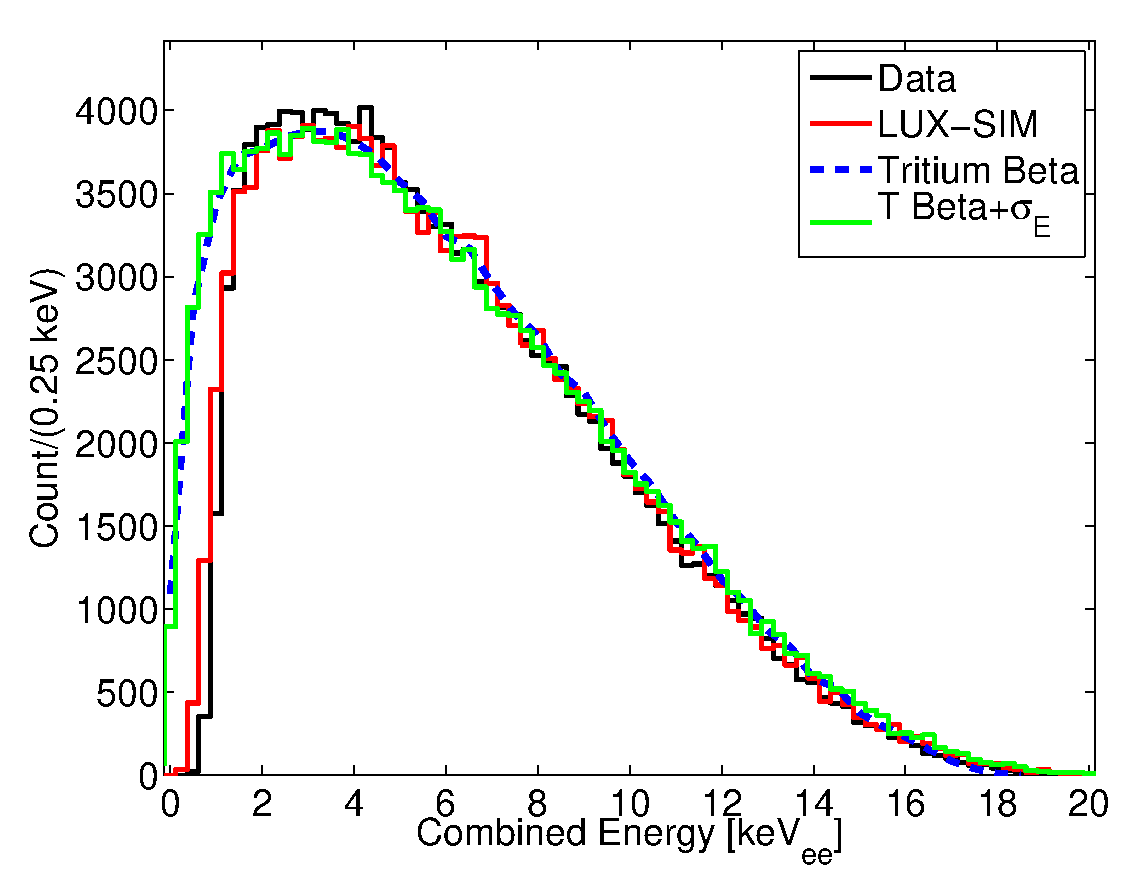
\includegraphics[width=73mm]{Chapter_E_Scale/Figures/E_Spec/E_spec_compare_SIM.eps}}
\hfill
\subcaptionbox{170 V/cm \label{fig:3b}}{\includegraphics[width=73mm]{Chapter_E_Scale/Figures/E_Spec/E_spec_compare_SIM_log_.eps}}

\bigskip

\subcaptionbox{100 V/cm \label{fig:3c}}{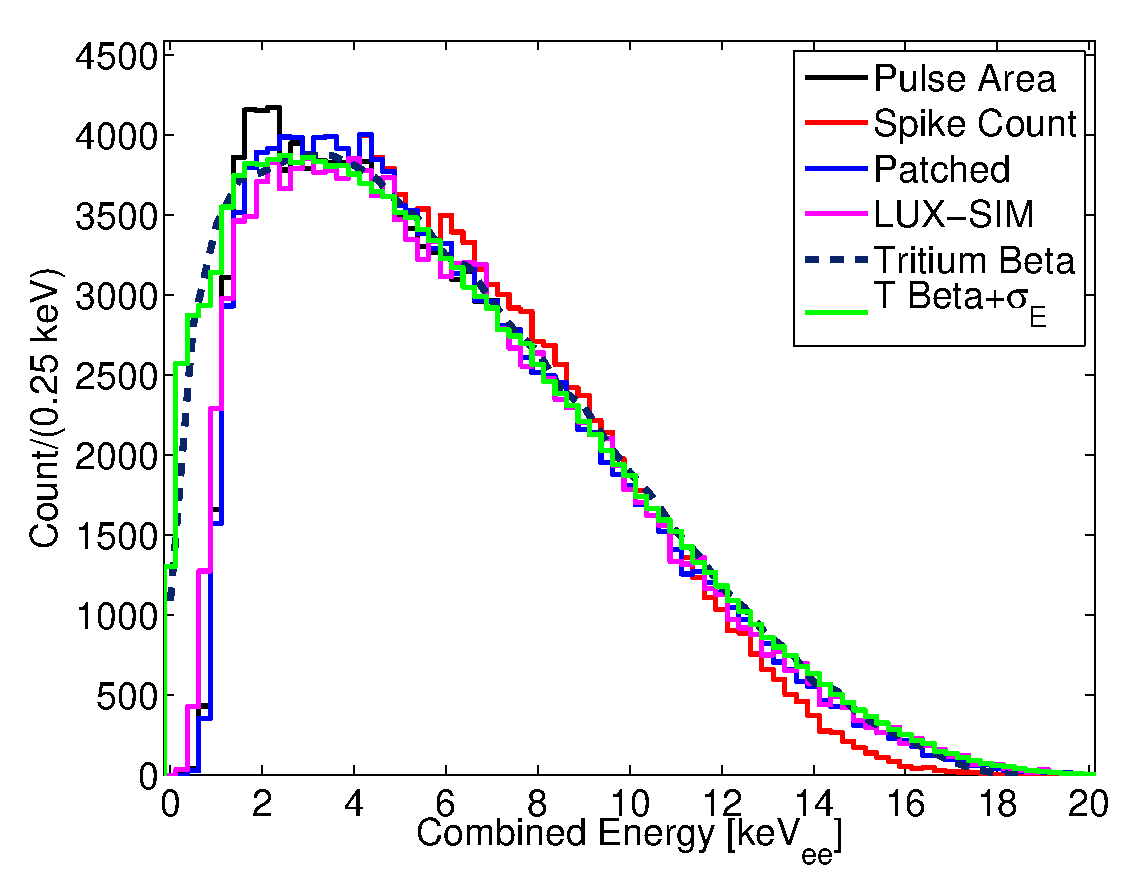
\includegraphics[width=73mm]{Chapter_E_Scale/Figures/Spec_Thresh_100/E_spec_compare_SIM.eps}}
\hfill
\subcaptionbox{100 V/cm \label{fig:3c}}{\includegraphics[width=73mm]{Chapter_E_Scale/Figures/Spec_Thresh_100/E_spec_compare_SIM_log_.eps}}

\caption{The tritium energy spectrum reconstructed from the data (black). Along with LUX SIM (blue), and the true tritium beta spectrum (blue) and a tritium spectrum smeared with detector resolution (green). }
\label{fig:E_spec}
\end{figure}

The reconstructed energy spectrum is in good agreement with the expected tritium beta spectrum with detector resolution, using both LUXSIM and the empirically determined resolution. The detector threshold reaches 100\% at about 1.5 keV, making the tritium beta peak clearly visible and providing crucial cross check of the reconstructed energy around the WIMP search region of interest (1-5 keV) and the model for energy given in equation \ref{eq:E_S1S2}. 

The 18.6 keV endpoint is another good low energy calibration point. We find that the end point of the reconstructed energy spectrum is consistent with that expected when convolving the true tritium beta spectrum with detector resolution. Though the energy scale for ER events was calibrated using mono-energetic sources well above the tritium Q value, the reconstructed tritium beta spectrum agrees with the expectation all the way down to the 1.5 keV threshold. The agreement at low energy is remarkable, considering we have reconstructed the energy scale for ER events by summing photons and electrons and ignoring the term lost to heat. We find that the modeling outlined in section \ref{sec:LXe_Theory} holds even at 1 $\rm keV_ee$.



Figure \ref{fig:Thres} shows the Energy threshold attained by comparing the data to the expected photon, electron and energy spectrum, at 170 and 100 V/cm. The energy threshold is set by the light collection of the much smaller S1 signal. For the energy threshold we find roughly 50\% efficiency at 1 $\rm keV_{ee}$ approaching 100\% at 1.5 $\rm keV_{ee}$ for both drift fields. The S1 and S2 detection threshold threshold will be discussed in Chapter \ref{Ch:LYQY}.


\begin{figure}[h!]\centering
\includegraphics[width=73mm]{Chapter_E_Scale/Figures/E_Spec/E_Thres_LY_QY_iter1.eps}
\includegraphics[width=73mm]{Chapter_E_Scale/Figures/Spec_Thresh_100/E_Thres_.eps}
\caption{Detector threshold calculated by comparing the data to the true tritium energy spectrum having applied detector resolution effects. Top: data with a drift field of 170 V/cm. Bottom: data with a drift field of 170 V/cm.}
\label{fig:Thres}
\end{figure}


\newpage

Figure \ref{fig:T_S2S1} shown the tritium spectrum in S2 vs. S1 space. Having calibrated the energy scale we can overlay contours of constant energy with respect to the axes.

\begin{figure}[h!]\centering
\includegraphics[width=100mm]{Chapter_E_Scale/Figures/T_new/S2S1_T_.png}
\caption{Tritium calibration data, plotting S2 vs. S1. The horizontal black lines represent contours of constant energy, labeled in $\rm keV$. }
\label{fig:T_S2S1}
\end{figure}


\section{Summery}

We have constrained the value of $\rm g_1$ and $\rm g_2$ to be 0.097 $\pm$ 0.008 and 5.75 $\pm$ 1.40 respectively. The final fit for the values of $\rm g_1$ and $\rm g_2$ is shown in figure \ref{fig:Doke2}. Comparing the value of the single electron size measured the LUX detector to $\rm g_2$, we find the electron extraction efficiency $\rm \epsilon$ to be  59.3 $\pm$14\%. The value for $\rm \epsilon$ is in good agreement with the expectation at the extraction field of 3.5 kV/cm. Having calibrated the combined energy scale using line sources above 40 keV we test the model of equation \ref{eq:E_S1S2} by reconstructing a tritium beta spectrum. We find that the tritium beta shape reconstructed in energy by counting photons and electrons is in good agreement with the true shape. Specifically, both the end point (18.6 keV) and the mode (3-4 keV) of the spectrum line up. By comparing the data to the tritium beta spectrum the detector energy threshold is found to be 50\% at 1 keV and approaching 100\% above 1.5 keV.


